\documentclass{article}
\usepackage[utf8]{inputenc}
% are all of these packages really necessary?
% no.
% i'm just too lazy to only grab the packages i want for a specific
% document, so i just glob all of my most commonly used packages together
% this is bad practice.
\usepackage{amsmath,amsthm,amssymb,amsfonts, fancyhdr, color, comment, graphicx, environ, mdframed, soul, calc, enumitem, mdframed, xcolor, geometry, empheq, mathtools, tikz, pgfplots, caption, subcaption, hyperref,multicol}

\usetikzlibrary{external}
\tikzexternalize[prefix=tikz/,optimize command away=\includepdf]

%tikzpicture
\usepackage{tikz}
\usepackage{scalerel}
\usepackage{pict2e}
\usepackage{tkz-euclide}
\usetikzlibrary{calc}
\usetikzlibrary{patterns,arrows.meta}
\usetikzlibrary{shadows}
\usetikzlibrary{external}

%pgfplots
\usepackage{pgfplots}
\pgfplotsset{compat=newest}
\usepgfplotslibrary{statistics}
\usepgfplotslibrary{fillbetween}
\usepgfplotslibrary{polar}

\tikzset{external/export=true}
\pgfplotsset{
    standard/.style={
    axis line style = thick,
    trig format=rad,
    enlargelimits,
    axis x line=middle,
    axis y line=middle,
    enlarge x limits=0.15,
    enlarge y limits=0.15,
    every axis x label/.style={at={(current axis.right of origin)},anchor=north west},
    every axis y label/.style={at={(current axis.above origin)},anchor=south east}
    }
}
\newcommand*\widefbox[1]{\fbox{\hspace{2em}#1\hspace{2em}}}
% Command "alignedbox{}{}" for a box within an align environment
% Source: http://www.latex-community.org/forum/viewtopic.php?f=46&t=8144
\newlength\dlf  % Define a new measure, dlf
\newcommand\alignedbox[2]{
% Argument #1 = before & if there were no box (lhs)
% Argument #2 = after & if there were no box (rhs)
&  % Alignment sign of the line
{
\settowidth\dlf{$\displaystyle #1$}  
    % The width of \dlf is the width of the lhs, with a displaystyle font
\addtolength\dlf{\fboxsep+\fboxrule}  
    % Add to it the distance to the box, and the width of the line of the box
\hspace{-\dlf}  
    % Move everything dlf units to the left, so that & #1 #2 is aligned under #1 & #2
\boxed{#1 #2}
    % Put a box around lhs and rhs
}
}

\hypersetup{
    colorlinks=true,
    linkcolor=blue,
    filecolor=magenta,      
    urlcolor=cyan,
    pdftitle={Homework 22 Solutions},
    pdfpagemode=UseOutlines,
    bookmarksopen=true,
    pdfauthor={Christina Phan}
}
\newcommand{\lrp}[1]{\left( #1 \right)}
\newcommand{\abs}[1]{\left\vert #1 \right\vert}
\newcommand{\lra}[1]{\left\langle #1 \right\rangle}
\newcommand{\lrb}[1]{\left[ #1 \right]}
\newcommand{\norm}[1]{\left\lVert #1 \right\rVert}
\newcommand{\iintR}[0]{\iint\limits_{R}}
\renewcommand{\u}[0]{\mathbf{u}}
\renewcommand{\i}[0]{\mathbf{i}}
\renewcommand{\j}[0]{\mathbf{j}}
\renewcommand{\k}[0]{\mathbf{k}}
\newcommand{\T}[0]{\mathbf{T}}
\newcommand{\N}[0]{\mathbf{N}}
\newcommand{\B}[0]{\mathbf{B}}
\renewcommand{\r}[0]{\mathbf{r}}
\renewcommand{\a}[0]{\mathbf{a}}
\renewcommand{\v}[0]{\mathbf{v}}
\newcommand{\F}[0]{\mathbf{F}}
\newcommand{\n}[0]{\mathbf{n}}
\newcommand{\eqq}[0]{\stackrel{?}{=}}
\renewcommand{\arraystretch}{1.25}

\geometry{letterpaper, portrait, margin=1in}
\renewcommand{\footrulewidth}{0.8pt}
\setlength\parindent{0pt}
\pagestyle{fancy}
\lhead{Christina Phan}
\rhead{MAT 21D} 
\chead{\textbf{Homework 22 Solutions}}

\newcommand{\Solution}{\textit{Solution}}
\pgfplotsset{compat=1.18}
\begin{document}

\phantomsection
\addcontentsline{toc}{section}{Problem 1 (Parts)}\textbf{Problem 1 (Parts)}

Consider the vector field $\F(x,y,z)=\lra{x,y,z}$.

\phantomsection
\addcontentsline{toc}{subsection}{1(a)}\textbf{(a)} Show that $\nabla \times \F=\mathbf{0}$.


\Solution

Since $\F(x,y,z)=\lra{x,y,z}$,
\begin{align*}
    \nabla \times \F&=\begin{vmatrix}\i & \j & \k\\ \frac{\partial}{\partial x} & \frac{\partial}{\partial y}& \frac{\partial}{\partial z}\\ x & y & z\end{vmatrix}\\
    &=\Bigg(\frac{\partial }{\partial y}(z)-\frac{\partial }{\partial z}(y)\Bigg)\i-\Bigg(\frac{\partial}{\partial x}(z)-\frac{\partial}{\partial z}(x)\Bigg)\j+\Bigg(\frac{\partial}{\partial x}(y)-\frac{\partial}{\partial y}(x)\Bigg)\k\\
    &-\lrp{0-0}\i-\lrp{0-0}\j+\lrp{0-0}\k\\
    &=\lrp{0}\i+\lrp{0}\j+\lrp{0}\k\\
    &=\lra{0,0,0}\\
    &=\mathbf{0}\tag{vector with all $0$'s is called the zero vector aka $\mathbf{0}$}
\end{align*}
\qed

\phantomsection
\addcontentsline{toc}{subsection}{1(b)}\textbf{(b)} Find a vector field with twice-differentiable components whose curl is $\F$ or prove that no such field exists.

\Solution

Let $\mathbf{G}(x,y,z)=\lra{M,N,P}$ where $\mathbf{G}$'s components are twice-differentiable.
\begin{align*}
    \nabla \times \mathbf{G} &=\begin{vmatrix}\i & \j & \k\\ \frac{\partial}{\partial x} & \frac{\partial}{\partial y}& \frac{\partial}{\partial z}\\ M & N & P\end{vmatrix}\\
    &=\Bigg(\frac{\partial }{\partial y}(P)-\frac{\partial }{\partial z}(N)\Bigg)\i-\Bigg(\frac{\partial}{\partial x}(P)-\frac{\partial}{\partial z}(M)\Bigg)\j+\Bigg(\frac{\partial}{\partial x}(N)-\frac{\partial}{\partial y}(M)\Bigg)\k\\
     &=\Bigg(\frac{\partial }{\partial y}(P)-\frac{\partial }{\partial z}(N)\Bigg)\i+\Bigg(-\frac{\partial}{\partial x}(P)+\frac{\partial}{\partial z}(M)\Bigg)\j+\Bigg(\frac{\partial}{\partial x}(N)-\frac{\partial}{\partial y}(M)\Bigg)\k\\
    &=\lra{\frac{\partial P}{\partial y}-\frac{\partial N}{\partial z}, -\frac{\partial P}{\partial x}+\frac{\partial M}{\partial z},\frac{\partial N}{\partial x}-\frac{\partial M}{\partial y}}
\end{align*}
If $\text{curl }\mathbf{G}=\nabla \times \mathbf{G} = \F$, then
\begin{align*}
    \nabla \times \mathbf{G} &= \F\\
    \lra{\frac{\partial P}{\partial y}-\frac{\partial N}{\partial z}, -\frac{\partial P}{\partial x}+\frac{\partial M}{\partial z},\frac{\partial N}{\partial x}-\frac{\partial M}{\partial y}}&=\lra{x,y,z}\\
    \implies \frac{\partial P}{\partial y}-\frac{\partial N}{\partial z}&=x\\
    \implies -\frac{\partial P}{\partial x}+\frac{\partial M}{\partial z}&= y\\
    \implies \frac{\partial N}{\partial x}-\frac{\partial M}{\partial y}&= z
\end{align*}
Since $\mathbf{G}$ has twice-differentiable components,
\begin{align*}
    \frac{\partial }{\partial x}\lrp{ \frac{\partial P}{\partial y}-\frac{\partial N}{\partial z}}=\frac{\partial }{\partial x}\lrp{x}&\implies \frac{\partial^2 P}{\partial x \partial y}- \frac{\partial ^2 N}{\partial x\partial z}=1\\
    \frac{\partial }{\partial y}\lrp{- \frac{\partial P}{\partial x}+\frac{\partial M}{\partial z}}=\frac{\partial }{\partial y}\lrp{y}&\implies -\frac{\partial^2 P}{\partial y \partial x}+ \frac{\partial ^2 M}{\partial y\partial z}=1\\
    \frac{\partial }{\partial z}\lrp{ \frac{\partial N}{\partial x}-\frac{\partial M}{\partial y}}=\frac{\partial }{\partial z}\lrp{z}&\implies \frac{\partial^2 N}{\partial z \partial x}- \frac{\partial ^2 M}{\partial z\partial y}=1
\end{align*}
Adding up the left and right hand sides, we get
\begin{align*}
    \lrp{\frac{\partial^2 P}{\partial x \partial y}- \frac{\partial ^2 N}{\partial x\partial z}}+\lrp{-\frac{\partial^2 P}{\partial y \partial x}+ \frac{\partial ^2 M}{\partial y\partial z}}+\lrp{\frac{\partial^2 N}{\partial z \partial x}- \frac{\partial ^2 M}{\partial z\partial y}}&=\lrp{1}+\lrp{1}+\lrp{1}\\
    \lrp{\frac{\partial ^2 P}{\partial x \partial y}-\frac{\partial ^2 P}{\partial y \partial x}}+\lrp{-\frac{\partial^2 N}{\partial x\partial z}+\frac{\partial^2 N}{\partial z\partial x}}+\lrp{\frac{\partial ^2 M}{\partial y\partial z}-\frac{\partial^2 M}{\partial z\partial y}}&=3\tag{rearrange}\\
    \lrp{0}+\lrp{0}+\lrp{0}&=3\tag{mixed second 
    partial derivatives are equal}\\
    0&=3
\end{align*}
Clearly, $0\neq 3$, so $\mathbf{G}(x,y,z)=\lra{M,N,P}$ does not exist.

Therefore, there is no such field that exists where the field's curl is $\F$.

\qed

\phantomsection
\addcontentsline{toc}{section}{Problem 2}\textbf{Problem 2}

Consider the surface cut from the paraboloid $4x^2+y+z^2=4$ by the $xz$-plane. If $\n$ is the normal vector pointing away from the origin and $\F$ is the vector field
\begin{equation*}
    \F(x,y,z)=\lra{-z+\frac{1}{2+x},\tan^{-1}(y),x+\frac{1}{4+z}}
\end{equation*}
set up an integral that evaluates $\displaystyle \iint_S\lrp{\nabla \times \F}\cdot \n\,d\sigma$ using a more favorable surface. Then use the substitution $u=2x$, $v=z$ to evaluate the integral.

\Solution

Recall that by Strokes' Theorem, $\displaystyle \iint_S \lrp{\nabla \times \F}\cdot\n\,d\sigma$ only depends on the boundary curve of $S$, not $S$ itself.

We can have our surface just be the paraboloid surface on the $xz$-plane. This new surface will still have the same boundary curve as the paraboloid surface.

Let's find $\displaystyle \iint_S \lrp{\nabla \times \F}\cdot\n\,d\sigma$ using the paraboloid surface on the $xz$-plane.

\phantomsection
\addcontentsline{toc}{subsection}{Curl}\textbf{Curl}

Since $\displaystyle
    \F(x,y,z)=\lra{-z+\frac{1}{2+x},\tan^{-1}(y),x+\frac{1}{4+z}}$,
\begin{align*}
   \nabla \times \F&=\begin{vmatrix}\i & \j & \k\\ \frac{\partial}{\partial x} & \frac{\partial}{\partial y}& \frac{\partial}{\partial z}\\ -z +\frac{1}{2x} & \tan^{-1}(y) & x+\frac{1}{4+z}\end{vmatrix}\\
    &=\Bigg(\frac{\partial }{\partial y}\lrp{ x+\frac{1}{4+z}}-\frac{\partial }{\partial z}(\tan^{-1}(y))\Bigg)\i-\Bigg(\frac{\partial}{\partial x}\lrp{ x+\frac{1}{4+z}}-\frac{\partial}{\partial z}\lrp{-z +\frac{1}{2x}}\Bigg)\j\\
    &\hspace{3em}+\Bigg(\frac{\partial}{\partial x}(\tan^{-1}(y))-\frac{\partial}{\partial y}\lrp{-z +\frac{1}{2x}}\Bigg)\k\\
    &=\lrp{0-0}\i -\lrp{1-(-1)}\j+\lrp{0-0}\k\\
    &=\lrp{0}\i-\lrp{2}\j+\lrp{0}\k\\
    &=\lrp{0}\i+\lrp{-2}\j+\lrp{0}\k\\
    &=\lra{0,-2,0}
\end{align*}

\phantomsection
\addcontentsline{toc}{subsection}{n dsigma}$\n\,d\sigma$

Since our surface is on the $xz$ plane, it's pretty easy to find $\n$. We know $\n$ is going to be on the $y$-axis (either $\j$ or $-\j$). Since we want to point \textit{away} from the origin, we know $\n = \j=\lra{0,1,0}$ (point up and away). If this explanation is not sufficient, please see Monday's (5/23) or today's (5/25) lecture.


Since $\nabla \times \F=\lra{0,-2,0}$ and $\n\,d\sigma = \lra{0,1,0}\,dA$,
\begin{align*}
    \iint_S \lrp{\nabla \times \F}\cdot \n\,d\sigma &= \iint_R \lra{0,-2,0}\cdot \lra{0,1,0}\,dA\\
    &=\iint_R 0(0) + (-2)(1) + 0(0)\,dA\\
    &=\iint_R -2 \,dA\\
    &=-2 \iint_R \,dA\tag{we can take constants out}
\end{align*}
\textbf{Region $R$}

Our region $R$ is the shadow of the surface on the $xz$-plane ($y=0$). That is, our region is $4x^2+0+z^2=4\implies 4x^2+z^2=4$.

Graphically, this is an ellipsoid that looks like
\begin{center}
\resizebox{3.5cm}{!}{
    \begin{tikzpicture}
    \begin{axis}[standard,
            xtick={-1,1},
            ytick={-2:2},
            samples=1000,
            xlabel={$x$},
            ylabel={$z$},
          xmin=-1.3,
          xmax=1.3,          
          ymin=-2.3,
          ymax=2.3,
            x=1cm,
            y=1cm/1,
           ]

    \node[anchor=center,label=south west:$O$] at (axis cs:0,0){};
\addplot[name path=F,domain={-1:1}]{sqrt(4-4*x^2)};
\addplot[name path=G,domain={-1:1}]{-sqrt(4-4*x^2)};
\addplot[fill=green, fill opacity=0.2] fill between [of=F and G, soft clip={domain=-1:1}];
    \end{axis}
    \end{tikzpicture}
}
\end{center}
Our lower and upper bounds for $z$ are $z=-\sqrt{4-4x^2}$ and $z=\sqrt{4-4x^2}$, respectively.

Our lower and upper bounds for $x$ are $x=-1$ and $x=1$, respectively.

Let's use the substitution $u=2x$, $v=z$ to evaluate the integral. 

Because we're using a substitution of variables, we'll need to throw in our Jacobian into the integral.

If you don't remember how to calculate the Jacobian, please see Homework 7 (campuswire \#25).

Our lower and upper bounds for $v$ are
\begin{align*}
    z=-\sqrt{4-4x^2}&\implies v = -\sqrt{4-4\lrp{\frac{u}{2}}^2}=-\sqrt{4-u^2}\tag{$u=2x\implies \dfrac{u}{2}=x$}\\
    z=\sqrt{4-4x^2}&\implies v = \sqrt{4-4\lrp{\frac{u}{2}}^2}=\sqrt{4-u^2}\tag{$u=2x\implies \dfrac{u}{2}=x$}
\end{align*}
Our lower and upper bounds for $u$ are
\begin{align*}
    x=-1&\implies \frac{u}{2}=-1\implies u = -2\tag{$u=2x\implies \dfrac{u}{2}=x$}\\
    x=1&\implies \frac{u}{2}=1\implies u = 2\tag{$u=2x\implies \dfrac{u}{2}=x$}
\end{align*}
Yes, our $xz$ region now turns into a circle of radius $2$ on the $uv$-plane. This fact will be helpful later.
\begin{center}
\resizebox{3.5cm}{!}{
    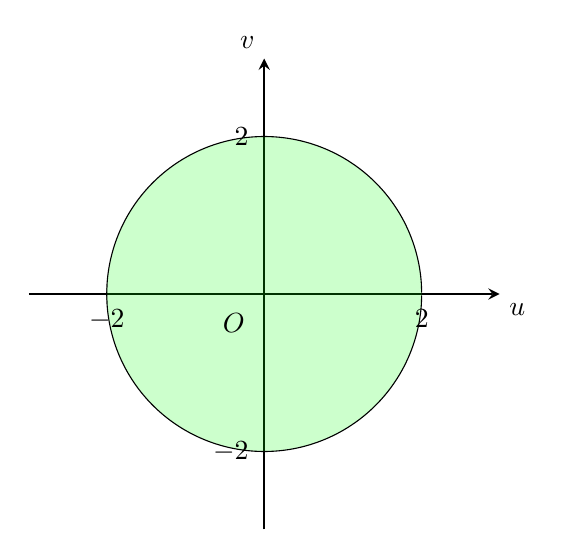
\begin{tikzpicture}
    \begin{axis}[standard,
            xtick={-2,2},
            ytick={-2,2},
            samples=1000,
            xlabel={$u$},
            ylabel={$v$},
          xmin=-2.3,
          xmax=2.3,          
          ymin=-2.3,
          ymax=2.3,
            x=1cm,
            y=1cm/1,
           ]

    \node[anchor=center,label=south west:$O$] at (axis cs:0,0){};
\addplot[name path=F,domain={-2:2}]{sqrt(4-x^2)};
\addplot[name path=G,domain={-2:2}]{-sqrt(4-x^2)};
\addplot[fill=green, fill opacity=0.2] fill between [of=F and G, soft clip={domain=-2:2}];
    \end{axis}
    \end{tikzpicture}
}
\end{center}
Let's calculate our Jacobian.
\begin{align*}
    \frac{\partial x}{\partial u}&=\frac{1}{2}\tag{$u=2x\implies \dfrac{u}{2}=x$}\\
    \frac{\partial x}{\partial v}&=0\\
    \frac{\partial z}{\partial u}&=0\\
    \frac{\partial z}{\partial v}&=1\\
    \begin{vmatrix}\frac{\partial x}{\partial u}&\frac{\partial x}{\partial v}\\ \frac{\partial z}{\partial u}&\frac{\partial z}{\partial v}\end{vmatrix}&=\begin{vmatrix}
    \frac{1}{2} & 0\\
    0 & 1
    \end{vmatrix}=\lrp{\frac{1}{2}}\lrp{1}-\lrp{0}\lrp{0}=\frac{1}{2}
\end{align*}
Let's go back to evaluating our integral.
\begin{align*}
    \iint_S \lrp{\nabla \times \F}\cdot \n\,d\sigma &= -2\iint_R \,dA\\
    &=-2\int_{-2}^2\int_{-\sqrt{4-u^2}}^{\sqrt{4-u^2}}\lrp{\frac{1}{2}}\,dv\,du\\
    &=-2\lrp{\frac{1}{2}}\int_{-2}^2\int_{-\sqrt{4-u^2}}^{\sqrt{4-u^2}}\,dv\,du\tag{we can take constants out}\\
    &=-\int_{-2}^2\int_{-\sqrt{4-u^2}}^{\sqrt{4-u^2}}\,dv\,du\\
    &=-\lrp{\text{area of circle}}\tag{$\displaystyle \int_{-2}^2\int_{-\sqrt{4-u^2}}^{\sqrt{4-u^2}}\,dv\,du$ is just area of region}\\
    &=-\lrp{\pi(2)^2}\\
    &=-\lrp{4\pi}\\
    &=\boxed{-4\pi}
\end{align*}



\phantomsection
\addcontentsline{toc}{section}{Problem 3}\textbf{Problem 3}

Suppose $\F$ is the curl of the vector field $\displaystyle\lra{y+\sqrt{z},e^{xyz},\cos xz}$.

\phantomsection
\addcontentsline{toc}{subsection}{3(a)}\textbf{(a)} Find the flux of $\F$ outward through the hemisphere $x^2+y^2+z^2=1$, $z\geq 0$.

\Solution

Recall that the flux of $\F$ outward through a surface is
\begin{equation*}
    \text{flux}=\iint_S \F\cdot \n \,d\sigma
\end{equation*}
By Strokes' Theorem,
\begin{align*}
     \text{flux}=\iint_S \F\cdot \n \,d\sigma=\oint_C \F\cdot d\r
\end{align*}
where $C$ is our boundary curve.

For the hemisphere $x^2+y^2+z^2=1$, the boundary curve would be when $z=0$. That is, the boundary curve would be $x^2+y^2+0^2=1\implies x^2+y^2=1$. 

Our boundary curve is the circle $x^2+y^2=1$ (circle of radius $1$).

We can parameterize this curve as $\r(t)=\lra{\cos t,\sin t, 0}$ where $0\leq t\leq 2\pi$ (go around entire circle counterclockwise).

We go counterclockwise around the circle because our flux is going \textit{outward}. By right hand rule, we also go counterclockwise around our boundary curve. If this explanation isn't sufficient, please see Monday's (5/23) or today's (5/25) lecture.

Since $\r(t)=\lra{\cos t,\sin t, 0}$,
\begin{align*}
    \F\lrp{\r(t)}&=\lra{\sin t +\sqrt{0},e^{(\cos t)(\sin t)(0)},\cos \lrp{\cos t(0)} }\\
    &=\lra{\sin t, e^0,\cos(0)}\\
    &=\lra{\sin t, 1, 1}\tag{$e^0=1$ and $\cos 0=1$}\\
    \r'(t)&=\lra{-\sin t, \cos t, 0}
\end{align*}
Let's evaluate the flux integral.
\begin{align*}
    \text{flux}&=\iint_S \F\cdot \n \,d\sigma \\
    &=\int_0^{2\pi}\lra{\sin  t,1,1}\cdot\lra{-\sin t,\cos t,0}\,dt\\
    &=\int_0^{2\pi}(\sin t)(-\sin t) + 1(\cos t) + 1(0)\,dt\\
    &=\int_0^{2\pi}-\sin^2 t + \cos t + 0\,dt\\
    &=\int_0^{2\pi} -\lrp{\frac{1}{2}\lrp{1 - \cos 2t}}+\cos t\,dt\tag{$\sin^2 t = \dfrac{1}{2}(1-\cos 2t)$}\\
    &=\int_0^{2\pi}-\lrp{\frac{1}{2}-\frac{1}{2}\cos 2t}+\cos t\,dt\\
    &=\int_0^{2\pi} -\frac{1}{2}+\frac{1}{2}\cos 2t + \cos t\,dt\\
    &=\lrb{-\frac{1}{2}t+\frac{1}{4}\sin 2t + \sin t}_0^{2\pi}\\
    &=\lrp{-\frac{1}{2}(2\pi)+\frac{1}{4}\sin 2(2\pi) + \sin 2\pi}-\lrp{-\frac{1}{2}(0)+\frac{1}{4}\sin 2(0)+\sin 0}\\
    &=\lrp{-\pi + \frac{1}{4}\sin 4\pi + \sin 2\pi}-\lrp{0+\frac{1}{4}\sin 0 + \sin 0}\\
    &=\lrp{-\pi + 0 + 0}-\lrp{0+0+0}\\
    &=\boxed{-\pi}
\end{align*}
\phantomsection
\addcontentsline{toc}{subsection}{3(b)}\textbf{(b)} Find the flux of $\F$ outward through the entire sphere $x^2+y^2+z^2=1$.

\Solution

If we're going through the entire sphere, then we can break up the flux into the sum of the upper and lower hemispheres' fluxes.

We already know what the upper hemisphere's flux is from (a).

The lower hemisphere's flux is pretty similar. We're just upside down.  Instead of going \textit{counterclockwise}, we go \textit{clockwise}.

Since we're going \textit{clockwise} instead of \textit{counterclockwise}, the lower hemisphere's flux will be the opposite of the upper hemisphere's flux. That is, the lower hemisphere's flux is $-(-\pi)=\pi$.

Our total flux is the sum of the upper and lower hemispheres' fluxes, so
\begin{equation*}
    \text{flux}=-\pi + \pi = \boxed{0}
\end{equation*}
\newpage
\phantomsection
\addcontentsline{toc}{section}{Problem 4}\textbf{Problem 4}

Let $\F$ be a vector field whose component functions have continuous derivatives on an open and connected region of space.

\phantomsection
\addcontentsline{toc}{subsection}{4(a)}\textbf{(a)} Which of the following statements imply or are implied by the other statements?

\renewcommand{\labelenumi}{\roman{enumiv}\roman{enumi}.}
\begin{multicols}{2}
\begin{enumerate}
      \item $\F$ is conservative
      \item $\displaystyle\oint_C \F\cdot d\r=0$ for any loops $C$
\columnbreak
\item $\F=\nabla f $ for some function $f$
\item $\nabla \times \F =0$
\end{enumerate}
\end{multicols}
\Solution

\phantomsection
\addcontentsline{toc}{subsubsection}{Recalls} \textbf{Recalls}

There are a few things we need to remember.
\renewcommand{\labelenumi}{\arabic{enumi}.}
\begin{enumerate}
    \item Recall that $\F$ is conservative if and only if $\displaystyle\oint_C \F\cdot d\r=0$ for \textbf{any} curve (loop) $C$.
    \item Recall that $\F$ is conservative if and only if $\F=\nabla f$ for some function $f$.
\item Recall from Homework 21 Problem 1(c) that if $\F(x,y,z)=\nabla f$ where $f$ has continuous second partial derivatives, then $\nabla \times \F=\mathbf{0}$.
\end{enumerate}


Based on all of these recalls, there are a couple of things we can conclude.

From Recall 1, we know statement i implies statement ii, and statement ii implies statement i because statement i and statement ii make up Recall 1 (``if and only if" so both ways).

From Recall 2, we know statement i implies statement iii, and statement iii implies statement i because statement i and statement iii make up Recall 2 (``if and only if" so both ways).

Therefore, statement ii and statement iii also imply each other.



From Recall 3, we know statement iii implies statement iv since statement iii and statement iv make up Recall 3.

\phantomsection
\addcontentsline{toc}{subsection}{4(b)}\textbf{(b)} What further condition do we need to impose on the region for the four statements to be equivalent?

\Solution

Recall that if $\F$ is a vector field on a \textit{simply} connected domain, then $\F$ is conservative if and only if $\nabla \times \F = \mathbf{0}$.

From this recall, we know that if our region is \textit{simply} connected, then statement i implies statement iv, and statement iv implies statement i (``if and only if" so both ways).


We can also see this using today's (5/25) lecture. 
If our region is \textit{simply} connected, then statement iv implies statement ii because if $\nabla \times \F = 0$, then by Stokes' Theorem
\begin{align*}
     \oint_C \F\cdot d\r = \iint_S \lrp{\nabla \times \F}\cdot \n\,d\sigma=\iint_S \mathbf{0}\cdot \n \,d\sigma = \iint_S 0\,d\sigma = 0
\end{align*}
We also know that statement ii implies statement i. If statement iv implies statement ii and statement ii implies statement i, then statement iv implies statement i.

Therefore, for the four statements to be equivalent, our region must be \textit{simply} connected (no holes).

\qed
\end{document}
